\documentclass{article}
\usepackage[final]{neurips}
\usepackage[framemethod=tikz]{mdframed}
\usepackage{lipsum}
\definecolor{mycolor}{rgb}{0.122, 0.435, 0.698}
\newmdenv[innerlinewidth=0.5pt, roundcorner=4pt,linecolor=mycolor,innerleftmargin=6pt,
innerrightmargin=6pt,innertopmargin=6pt,innerbottommargin=6pt]{mybox}
\usepackage[utf8]{inputenc} % allow utf-8 input
\usepackage[T1]{fontenc}    % use 8-bit T1 fonts
\usepackage[hidelinks]{hyperref}       % hyperlinks
\usepackage{url}            % simple URL typesetting
\usepackage{booktabs}       % professional-quality tables
\usepackage{amsfonts}       % blackboard math symbols
\usepackage{nicefrac,tcolorbox}       % compact symbols for 1/2, etc.
\usepackage{amsmath}
\usepackage{mdframed}
\usepackage{enumitem}
\usepackage{microtype}      % microtypography
\usepackage{graphicx,caption,xcolor}
\usepackage{mathtools}
\usepackage{xepersian}
\settextfont{XB Niloofar}
\setdigitfont{XB Niloofar}
\raggedbottom


\title{
	\vspace{-0.8em}
تمرین سری سوم درس نظریه گروه‌ها - دکتر رضاخانی
\\
{\normalsize
\textbf{مهلت تحویل:
جمعه ۱۷ فروردین ماه سال ۱۴۰۳ تا ساعت 59:23
\\
\vspace{-0.4em}
از طریق سامانه
\href{https://cw.sharif.edu/}{درس‌افزار شریف}
}
}
\vspace{-0.6em}
}

\usepackage[utf8]{inputenc}

\usepackage[english]{babel}
\setlength{\parindent}{3.5em}
\setlength{\parskip}{0.5em}
\renewcommand{\baselinestretch}{1.0}

\usepackage{calrsfs}
\DeclareMathAlphabet{\pazocal}{OMS}{zplm}{m}{n}
\newcommand{\La}{\mathcal{L}}
\newcommand{\Lb}{\pazocal{L}}


\newtcolorbox{boxes}[3][]
{
	colframe = #2!25,
	colback  = #2!10,
	coltitle = #2!40!black,  
	title    = {\textbf{#3}},
	#1,
}

\newenvironment{exercise}[3][\unskip]{%
	\par
	\noindent
	\textbf{تمرین
		#1
		[#2 امتیاز] 
		\def\temp{#3}\ifx\temp\empty
		: 
		\else
		: #3 \vspace{0.5em} \\ \noindent
		\fi
}}{}

\author{
حسین محمدی\\
  \lr{
  		\href{mailto:hossein.mohammadi.00427@gmail.com}{\texttt{	hossein.mohammadi.00427@gmail.com}}} \\
  \And
  زهرا کبیری\\
 \lr{
  		\href{mailto:kabiri.zahra98@gmail.com}{ \texttt{kabiri.zahra98@gmail.com}}}\\
  }

\begin{document}


\begin{minipage}{0.1\textwidth}% adapt widths of minipages to your needs
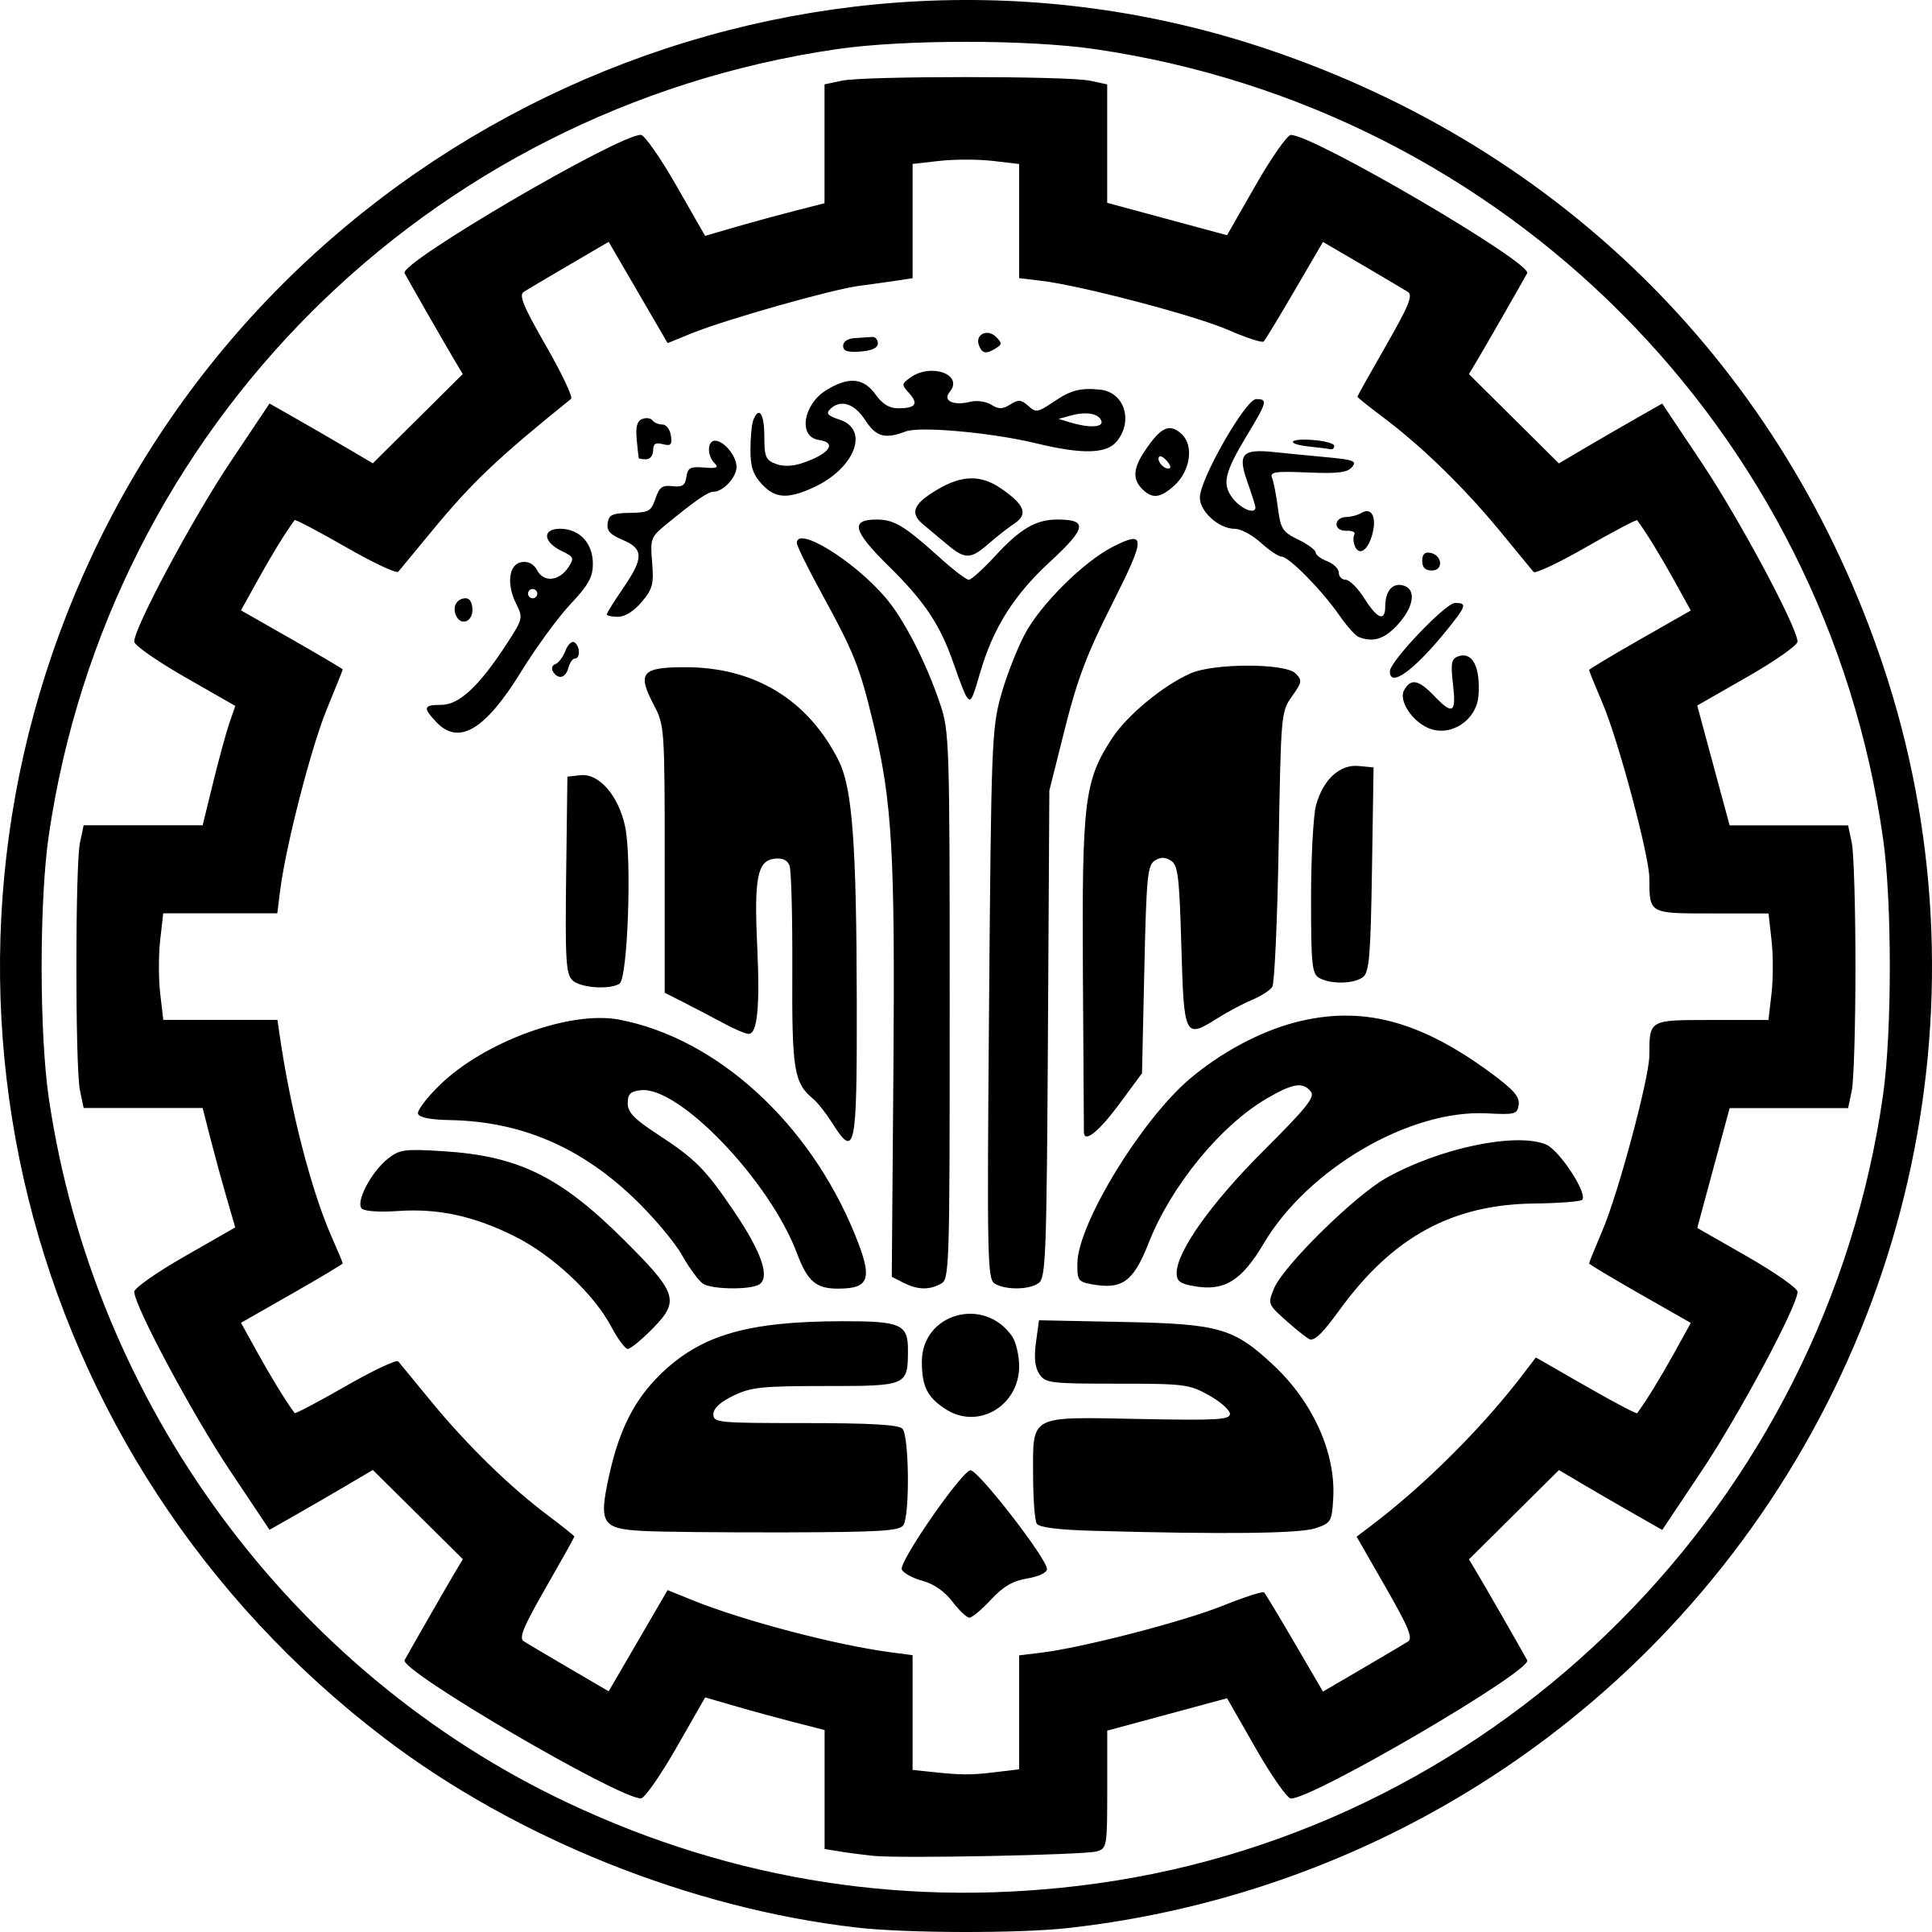
\includegraphics[width=1.1cm]{sharif-logo.png}
\end{minipage}%
\hfill%
\begin{minipage}{0.9\textwidth}\raggedleft
دانشگاه صنعتی شریف\\
زمستان ۱۴۰۲ - بهار ۱۴۰۳\\
\end{minipage}

\makepertitle

\begin{exercise}[10]{20}{گروه دور‌ی }
	الف) یک گروه دوری
	\LTRfootnote{Cyclic group} 
	از مرتبه 
	$n$، 
	چند مولد دارد؟
	(
	می‌گوییم
	$b\in G$ 
	یک مولد است و می‌نویسیم
	$G = \left < b \right >$
	 اگر گروه دوری 
	$G$ 
	،
	از توان‌های عضو $b$ ساخته شود.) 
	
	\noindent
	\vspace{0.25em}
	ب) گروه‌های دوری 
	$A$ 
	و 
	$B$ 
	را در نظر بگیرید که به ترتیب از مرتبه 
	$m$ 
	و 
	$n$ 
	هستند. نشان دهید که ضرب دکارتی این دو گروه ،
	$A \times B$ 
	دوری است اگر و فقط اگر 
	$m$ 
	و 
	$n$ 
	نسبت به هم اول باشند.
	\\
	
\end{exercise}


\begin{exercise}[11]{20}{همدسته‌ها و خواصشان}
	الف) فرض کنید 
	$H$ 
	زیرگروهی از یک گروه 
	$G$ 
	باشد. نشان دهید هر همدسته چپ از 
	$H$ 
	یک همدسته راست از زیرگروهی از 
	$G$ 
	است. آیا هر همدسته چپ 
	$H$، 
	همدسته راستی از 
	$H$ 
	هست؟ برای پاسخ خود دلیلی بیاورید.
	
	\noindent
	\vspace{0.25em}
	ب)  
	$H$ 
	یک زیرگروه از 
	$G$ 
	است به طوری که حاصل ضرب هر دو همدسته راست 
	$H$ 
	دوباره یک همدسته راست از 
	$H$ 
	است
	\footnote{منظور از ضرب دو‌ همدسته، ضرب درونی است. برای دو همدسته‌ی  
	$Hg_1$ و $Hg_2$ از  $H\leq G$ ضرب درونی به این شکل تعریف می‌شود:
	\[
	Hg_1Hg_2 = \{h_1g_1h_2g_2 \; | \; \forall h_1,h_2\in H \}
	\]
	}
	. نشان دهید که برای هر 
	$h \in H$ 
	و هر 
	$g\in G$
	داریم
	\footnote{از خانم حانیه ملکی و آقای ارمیا هلالی برای تذکر دادن این اشتباه تایپی سپاسگزاریم.}
	:
	\begin{equation*}
		ghg^{-1} \in H
	\end{equation*}
\end{exercise}


\begin{exercise}[12]{10}{گروه تبدیلات خطی فضای اقلیدسی}
	\vspace{-1em}
	\begin{boxes}{black}{تعریف گروه‌ تبدیلات خطی:}
		مجموعه تبدیلات خطی وارون‌پذیر روی 
		$\mathbb{R}^n$ 
		را گروه 
		$GL_n(\mathbb{R})$ 
		می‌نامیم
		\footnote{این سرواژه از 
			\lr{{\color{red} G}eneral {\color{red} L}inear group}
			وام گرفته شده است.
		}
		. به عنوان مثال برای 
		$n=2$ 
		ماتریس 
		$A_{2 \times 2}$ 
		، یک عضو از 
		$GL_2(\mathbb{R})$ 
		است.
		\begin{equation*}
			A_{2 \times 2} = \left[\begin{matrix}0&1\\1&0\\\end{matrix}\right]
		\end{equation*}
		حالا اگر زیرمجموعه‌ای از این تبدیلات خطی وارون‌پذیر را در نظر بگیریم که دترمینان آن‌ها برابر با ۱ است به گروهی می‌رسیم که به آن 
		$SL_n(\mathbb{R})$ 
		می‌گوییم
		\footnote{این سرواژه از  
			\lr{{\color{red} S}pecial {\color{red} L}inear group}
			وام گرفته شده است.
		}
		. 
	\end{boxes} 
	\noindent
	\vspace{0.7em}
	برای عدد حقیقی 
	$r \neq 0$، 
	مجموعه 
	$A_r$ 
	را این‌طور معرفی می‌کنیم:
	\begin{equation*}
		A_r= \{A\in GL_n(\mathbb{R})  \;|\;  \det A =r\}
	\end{equation*}
	
	\noindent
	الف) نشان دهید 
	$A_r$ 
	یک همدسته چپ 
	$SL_n(\mathbb{R})$ 
	است. 

\noindent
\vspace{0.25em}
	ب) آیا هر همدسته چپ 
	$SL_n(\mathbb{R})$ 
	را می‌توان به صورت 
	$A_r$ 
	نوشت؟ (برای یک 
	$r\neq 0$
	)
	\\
\end{exercise}
\begin{exercise}[13]{20}{گروه چندوجهی و مولدهایش}
	در این تمرین قصد داریم گروه چندوجهی را به کمک مولدهایش معرفی کنیم. در کلاس دیده‌اید که گاهی هیچ قیدی روی مولدها نیست و گروه تولید شده، «گروه آزاد» نامیده می‌شود. در اینجا روی مولدهای گروه 
	$D_n$
	قیودی داریم.
	
	\noindent
	مجموعه 
	$G$ 
	را در نظر بگیرید که اعضای آن تمام 
	$x^i y^j$هایی هستند که 
	$i,j \in \{0,1,2,...,n-1\}$. 
	همچنین فرض می‌کنیم این خاصیت‌ها را دارند
	\footnote{در مورد خاصیت دوم،  
	می توانیم با شرط 
	$0\leq i,i' <2$  و 
	$0 \leq j,j' < n$
	آن را به شکل 
	$i=i'$
	و
	$j=j'$
	بنویسیم.
	
	منظور از $a \stackrel{n}{\equiv} b$‌این است که 
	$n|(a-b)$
	یا $a$ و $b$ در تقسیم بر $n$ هم‌باقی‌مانده هستند. 
	
	 از آقای پویا حسینی برای تذکر این نکته ممنونیم. با هرکدام از این قراردادها که راحت‌تر هستید کار کنید.
	}:
	\begin{equation*}
		\begin{aligned}
			&x^2=y^n=e \;\;\;\;\;\; ; \;\;\;\;\;\; n>2\\
			&x^i y^j =x^{i'} y^{j'} \Longleftrightarrow i \stackrel{2}{\equiv} i', j \stackrel{n}{\equiv} j'\\
			&xy=y^{-1}x
		\end{aligned}
	\end{equation*}
	الف) حاصل ضرب 
	$(x^i y^j)(x^k y^l)$ 
	را می‌توان به صورت 
	$x^{\alpha}y^{\beta}$ 
	نوشت. 
	$\alpha$
	و
	$\beta$
	را بیابید. 
	
	\noindent
	ب) نشان دهید که 
	$G$ 
	یک گروه ناجابه‌جایی از مرتبه 
	$2n$ 
	است. 
	
	\noindent
	ج) 
	$Z(G)$ ،
	مرکز
	\LTRfootnote{Center} 
	گروه 
	$G$ 
	را این‌طور معرفی می‌کنیم:
	\begin{equation*}
		Z(G)=\{z\in G \;\big| \; zg=gz  \;\;\; , \;\;\; \forall g \in G \}
	\end{equation*}
	اگر 
	$n$ 
	فرد باشد نشان دهید که مرکز
	$G$، 
	بدیهی است؛ یعنی $Z(G) = \{e\}$. 
	\\
	همچنین نشان دهید اگر 
	$n$ 
	زوج باشد مرکز این گروه نابدیهی است؛ یعنی اعضایی به غیر از
	$e$ 
	دارد.
	\\
	یک گروه با این ویژگی‌ها یک گروه چندوجهی  \LTRfootnote{Dihedral group}
	نام دارد. می‌توانیم آن را به روش هندسی این‌طور توصیف کنیم. 
	\\
	\begin{mdframed}
			
		عضو
		$y$ 
		را یک دوران به زاویه 
		$\frac{2\pi}{n}$ 
		حول مبدا مختصات در نظر می‌گیریم. عضو
		$x$ 
		را نیز یک انعکاس نسبت به محور عمودی در نظر می‌گیریم. 
		گروهی که از حاصل ضرب این مولدها با قید‌های داده شده به دست می‌آيد همان گروه 
		$D_n$ 
		است.
	\end{mdframed}
\end{exercise}

\begin{exercise}[۱۴]{30}{بافتن گیسوها!}
	در این تمرین با گیسوها، ضربشان و خواص گروهی‌شان بیشتر آشنا می‌شویم.
	
	\noindent
	حتما تا الان با نمایش تصویری اعضای گروه گیسو آشنا شده‌اید. دو عضو 
	$\sigma_1 = \vcenter{\hbox{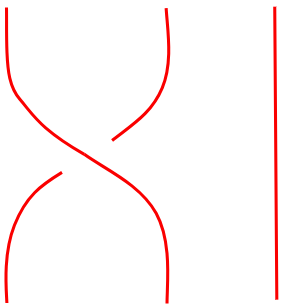
\includegraphics[height= 4.0 em]{Pics/g1.png}}}$
	و
	$\sigma_2 = \vcenter{\hbox{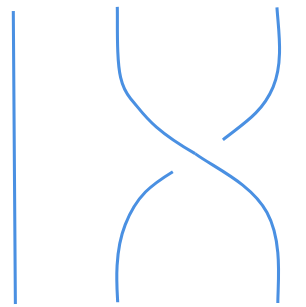
\includegraphics[height= 4.0 em]{Pics/g2.png}}}$
	از گروه 
	$B_3$
	را در نظر بگیرید؛ ضرب آنها با در امتداد هم قرار دادن این دو گیسو ساخته می‌شود.
	
	\begin{figure}[h]
		\centering
	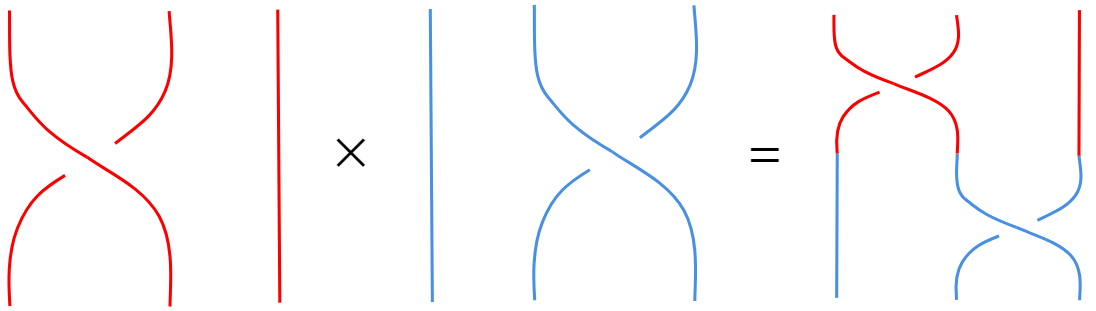
\includegraphics[scale=.5]{Pics/g3.png}
		\caption*{شکل ۱: نحوه ضرب کردن دو عضو از گروه گیسو}
	\end{figure}
	
	\noindent
	الف) گروه‌گیسو تعمیمی از گروه جایگشت است. یک همریختی بین گروه گیسو
	$B_n$
	و گروه جایگشت‌ها
	$S_n$
	 تعریف کنید و همچنین هسته‌ی این همریختی را نشان دهید. (در تعریف و معرفی هسته‌ی همریختی، نمایش تصویری بالا بهره ببرید و خیلی برای اثبات‌ها به خود زحمت ندهید؛ بسیاری از خواص گروه $B_N$ هنوز هم که هنوز است اثبات نشده‌اند.)
	 
	 \vspace{0.25em}
	 \noindent
	 ب) به شکل تصویری نشان دهید که دو عضو 
	 $\sigma_1$
	 و 
	 $\sigma_2$
	 مولدهای گروه 
	 $B_3$
	 هستند.
	 
	  \vspace{0.25em}
	 \noindent
	 ج) گروه گیسو‌ی مرتبه‌ی سه، گروه آزاد نیست. بین مولدهایش قیدی وجود دارد. این قید را به‌دست آورید. (راهنمایی: ضرب‌های سه‌تایی مولدها را در نظر بگیرید و ببینید که کدام دو ضرب سه‌مولدی با هم برابرند.)
	 
	   \vspace{0.25em}
	 \noindent
	 د) در این بخش به سراغ مرکز گروه می‌رویم. نشان دهید که گیسوی شکل
	 2
	  با چند عضو نوعی (حداقل سه عضو) از گروه 
	 $B_3$
	 جابه‌جا می‌شود.
	 
	 
	
		\begin{figure}[h]
		\centering
		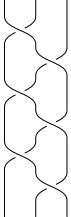
\includegraphics[scale=1.1]{Pics/g4.png}
		\caption*{شکل 2: گیسوی
			$(\sigma_1\sigma_2)^3$
			 که با تمامی گیسو‌های دیگر جابه‌جا می‌شود.}
		\label{barid2}
	\end{figure}
	\noindent
	 به طور کلی می‌شود نشان داد که مرکز گروه 
	$B_N$ به شکل زیر است:
	\[
	Z(B_N) = \left < (\sigma_1 \dots \sigma_{N-1})^N\right >
	\]

\noindent
گروه گیسو در فیزیک دوبعدی بسیارمهم است و در جعبه‌ی صفحه‌ی بعد به اهمیت آن پرداخته‌ایم.
	
	
	 
	
\end{exercise}


















\newpage

\begin{boxes}{black}{آمار ذرات و ارتباط با گروه‌های جایگشت و گیسو}
	یکی از جالب‌ترین و فیزیکی‌ترین ارتباط‌ها بین ذرات و نظریه‌گروه‌ها، ارتباط بین اسپین ذرات و آمار آنهاست
	\footnote{ارتباط جالب توجه دیگر، ارتباط بین اسپین و نمایش‌های گروه پوانکاره است.
	همچنین در قضیه‌ی 
	\lr{CPT}
	هم نقش گروه‌ها و نمایش‌ها به شکل خیره‌کننده‌ای قابل ملاحظه است.
	}
	.
	
	علت این‌که گروه جایگشت در مکانیک کوانتومی (و حتی کلاسیک، در پارادوکس گیبس) مهم است، تمییزناپذیری ذرات است.
	
	حتما از درس مکانیک کوانتومی ۲ می‌دانید که فضای پیکربندی 
	$-N$ذره
	در $-d$بعد فضایی، 
	\[X^N = \underbrace{\mathbb{R}^d \times \dots \times \mathbb{R}^d}_{\text{\lr{N times}}}\]
	نیست؛ بلکه تمییزناپذیری ذرات قیدی روی این فضا می‌گذارد.
	
	عضو
	$\sigma \in S_N$
	از گروه جایگشت $N$ شی را در نظر بگیرید. مطابق توقع فیزیکی ما، دو نقطه‌ی زیر از فضای پیکربندی معادلند:
	\[
	(\vec{\textbf{x}}_1, \vec{\textbf{x}}_2 , \dots , \vec{\textbf{x}}_N ) \sim (\vec{\textbf{x}}_{\sigma(1)}, \vec{\textbf{x}}_{\sigma(2)} , \dots , \vec{\textbf{x}}_{\sigma(N)} )
	\] 


پس باید نقاطی از فضا را که با اعضای گروه جایگشت به هم مرتبط می‌شوند، یکسان در نظر بگیریم. بنابراین فضای پیکربندی فیزیکی 
\[
\mathfrak{X} = 
\frac{X^N}{S_N}
\]
است.


ارتباط بین آمار ذرات و گروه‌ جایگشت و گیسو از همین فضای پیکربندی نشات می‌گیرد، اما نیاز به کمی فرمالیسم هست که این رابطه‌ شفاف‌تر شود.

\textbf{برای مطالعه بیشتر:}
ارتباط آمار ذرات به فضای پیکربندیشان از طریق فرمول‌بندی انتگرال‌مسیر تک‌ذره‌ای روشن می‌شود. برای محاسبه‌ی انتگرال‌مسیر تک‌ذره‌ای، نیاز است که روی همه‌ی مسیرهای غیرهم‌ارز
\footnote{منظور مسیرهایی است که با یک نگاشت پیوسته به هم تبدیل نمی‌شوند.}
با وزن خاصی جمع زده شود:
\[
K = \sum_{\alpha \in \pi_1(\mathfrak{X})} \chi(\alpha) K^\alpha
\]
در رابطه‌ی بالا، $K$ انتشارگر ذره، $K^\alpha$ انتشارگر با مسیرهای در کلاس هموتوپی $\alpha$ و $\chi$ نمایش یک‌بعدی
\footnote{با نمایش‌ گروه‌ها در آینده آشنا می‌شوید.}
 گروه 
 $\pi_1(\mathfrak{X})$
 است.

می‌شود دید که گروه‌هموتوپی فضای 
$\frac{X^N}{S_N}$
برای ابعاد فضایی سه ‌به بالا، گروه 
$S_N$
و  برای فضاهای دو‌بعدی
$B_N$
(گروه گیسو) است.

\[
\pi_1(\mathfrak{X}) = \pi_1 \big( \frac{X^N}{S_N} \big) = \begin{cases}
	B_N & d=2\\
	S_N & d>2
\end{cases} 
\]
همچنین نمایش‌های یکانی و یک‌بعدی گروه جایگشت، تنها 
$\chi^+$
 (برای بوزون) و
  $\chi^-$
  (‌برای فرمیون) است
\footnote{
	منظور از 
	$\chi^+$
	 نمایش بدیهی است که برای هر عضو از $S_N$ مقدارش یک است. همچنین نمایش 
	 $\chi^-$
	 به ازای جایگشت‌های زوج مقدارش
	 $+1$
	 و برای جایگشت‌های فرد مقدارش 
	 $-1$
	 است.
	}
. اما گروه گیسو نمایش‌های یک بعدی بسیار متنوع‌تری دارد
\footnote{
مثلا چون گروه
$B_2$
(مربوط به فضای ‌پیکربندی دوذره‌ای در دو بعد) با گروه 
$\mathbb{Z}$
یکریخت است؛ یک نمایش یک‌بعدی و یکانی به شکل 
$\rho(n) = e^{in\theta}$
برای هر
$\theta \in \mathbb{R}$
دارد.
}
.


این تفاوت در گروه هموتوپی‌، آمارهای متنوعی در دو بعد را به همراه دارد که به طور کلی نام 
\lr{Anyon}
به آنها اطلاق می‌شود. برای سه‌بعد فضایی یا بالاتر، تنها دو آمار بوزونی و فرمیونی وجود دارد.

من قبلا یادداشتی در این مورد نوشته بودم، آن را روی سامانه بارگذاری می‌کنم تا برای مطالعه بیشتر آن را بخوانید.

\end{boxes}

 \end{document}
